%!TEX root = main.tex

\chapter{Fonctions à plusieurs variables}
\label{chapter:fonction2var}


Jusqu'à présent, nous avons considéré les fonctions comme des \textbf{fonctions à une seule variable}.
Ceci signifie qu'à une valeur $x$ pris dans $\mathbb{R}$ on associe une valeur $y=f(x)$, également dans $\mathbb{R}$. 
Nous nous intéressons maintenant à des fonctions à deux variables qui associent un couple de valeurs $(x,y)$ pris dans $\mathbb{R}\times\mathbb{R} = \mathbb{R}^2$ à une valeur $f(x,\,y)$ dans $\mathbb{R}$. On notera :
%
$$
\begin{aligned}
f:\mathcal{D}_f \subset \mathbb{R}^2 & \longmapsto \mathbb{R} \\
 (x,y) & \longmapsto z = f(x,\,y)
\end{aligned}
$$


\begin{comment}
Schéma d'interprétation (à faire avec l'enseignant)
%
\ifthenelse{\equal{\showDrawings}{1}}{
\begin{center}
\includegraphics[height=6cm]{figs/surf3D.png}
\end{center}
}{\vspace*{6cm}}
\end{comment}


Le domaine de définition $\mathcal{D}_f$ de la fonction $f(x,\,y)$ est l'ensemble des couples de valeurs $(x,y)$ où la valeur $z=f(x,\,y)$ est définie (c'est-à-dire, ``existe''). On représente ce domaine sur le plan $(x,y)$



\begin{exo}

\noindent \ding{45} Pour chacune des fonctions $f(x,\,y)$ suivantes, représenter son domaine de définition dans le plan $Oxy$.

\begin{tasks}(2)
\task $f(x,\,y) = \displaystyle \frac{x^3y + xy^2}{x+y}$
\task $f(x,\,y) = \sqrt{xy}$
\task $f(x,\,y) = \displaystyle \ln \left(1+\frac{x}{y}  \right)$
\task $f(x,\,y) = \displaystyle \frac{\ln x}{x^2+y^2-9}$
\end{tasks}
\end{exo}


\begin{sol}

\begin{tasks}(1)

\task $f(x,\,y) = \displaystyle \frac{x^3y + xy^2}{x+y}$ n'est pas définie si $x+y=0$, donc si $y=-x$.
%
\begin{center}
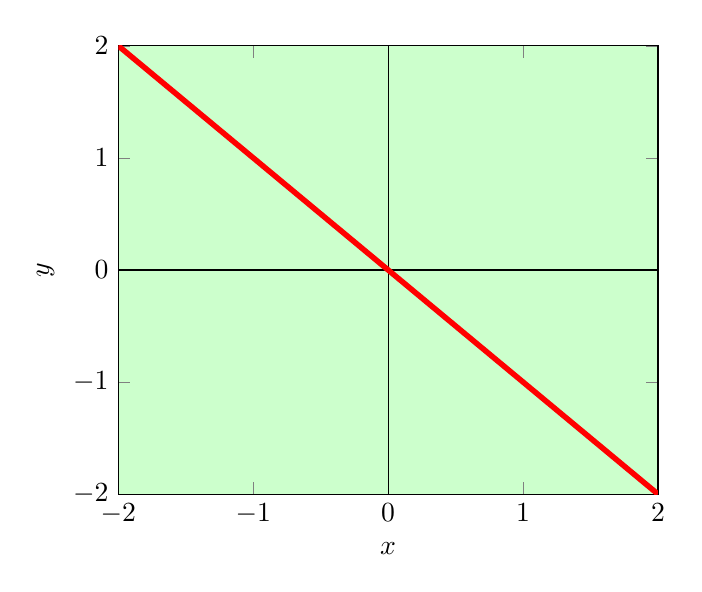
\begin{tikzpicture}
\begin{axis}[xmin=-2,xmax=2,ymin=-2,ymax=2,axis background/.style={fill=green!20},xlabel=$x$,ylabel=$y$]
\draw (-2,0) -- (2,0);
\draw (0,-2) -- (0,2);
\draw[red,line width=2pt] (-2.0,2.0) -- (2.0,-2.0);
\end{axis}
\end{tikzpicture}
\end{center}


\task $f(x,\,y) = \sqrt{xy}$ est définie ssi $xy \geq 0$, donc si $x$ et $y$ sont de signes opposés.
%
\begin{center}
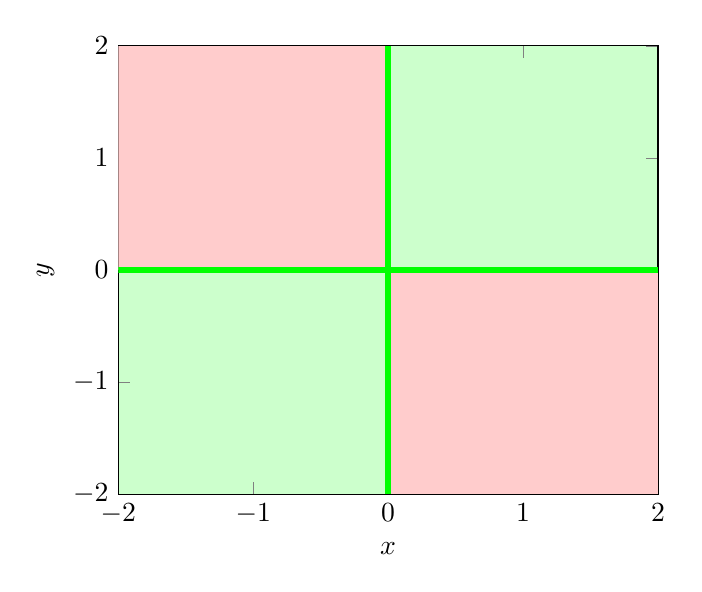
\begin{tikzpicture}
\begin{axis}[xmin=-2,xmax=2,ymin=-2,ymax=2,axis background/.style={fill=green!20},xlabel=$x$,ylabel=$y$]
\filldraw [fill=red!20, draw=none] (-2,2) rectangle (0,0);
\filldraw [fill=red!20, draw=none] (2,-2) rectangle (0,0);
\draw[green,line width=2pt] (-2,0) -- (2,0);
\draw[green,line width=2pt] (0,-2) -- (0,2);
\end{axis}
\end{tikzpicture}
\end{center}


% c
\task $f(x,\,y) = \displaystyle \ln \left(1+\frac{x}{y} \right)$ n'est définie que si $\frac{x}{y} > -1$ avec $y\ne0$.
%
\begin{center}
\begin{tikzpicture}
\begin{axis}[xmin=-2,xmax=2,ymin=-2,ymax=2,axis background/.style={fill=green!20},xlabel=$x$,ylabel=$y$]
\addplot[name path=B,domain=-2:2] {-x};
\addplot[name path=A,domain=-2:2] {0};
\tikzfillbetween[of=A and B]{red!20};
\addplot[domain=-2:2,red,line width=2pt] {-x};
\addplot[domain=-2:2,red,line width=2pt] {0};
\end{axis}
\end{tikzpicture}
\end{center}

% d
\task $f(x,\,y) = \displaystyle \frac{\ln x}{x^2+y^2-9}$ est définie lorsque $x>0$ et $x^2+y^2-9 \ne 0$.
%
\begin{center}
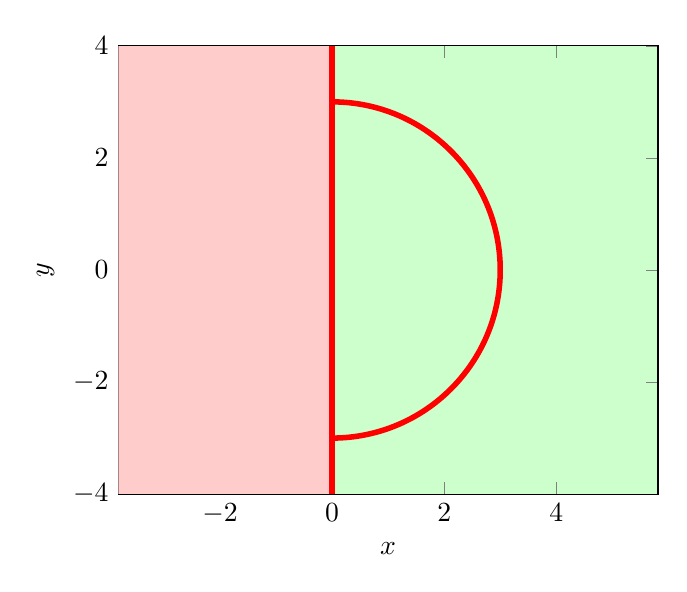
\begin{tikzpicture}
\begin{axis}[axis equal,xmin=-2,xmax=4,ymin=-4,ymax=4,axis background/.style={fill=green!20},xlabel=$x$,ylabel=$y$]
\filldraw [fill=red!20, draw=none] (-5,-4) rectangle (0,4);
\draw[red,line width=2pt] (0,-4) -- (0,4);
\draw[red,line width=2pt] (0,-3) arc [start angle=-90, end angle=90, radius=3];
\end{axis}
\end{tikzpicture}
\end{center}

\end{tasks}

\end{sol}

%%%%%%%%%%%%%%%%%%%%%%%%%%%%%%%%%%%%%%%%%%%%%%%%%%%%%%%%%%%%%%%%%%%%%%%%%%%%%%%%
\needspace{5cm}
\section{Calcul de dérivées partielles}

La dérivée partielle d'une fonction de plusieurs variables est sa dérivée par rapport à l'une de ses variables, les autres étant gardées constantes. Par exemple, prenons la fonction :
$$f(x,\,y) = x^2 \cos(y)$$
La dérivée par rapport à $x$ est :
$$
\displaystyle \frac{\partial}{\partial x} f(x,\,y) = 2x \cos(y)
$$
et la dérivée par rapport à $y$ est:
$$
\displaystyle \frac{\partial}{\partial y} f(x,\,y) = -x^2 \sin(y)
$$

On a donc considéré $\cos(y)$ comme une constante lors de la dérivation par rapport à $x$, et c'est $x^2$ qui a été considérée comme une constante lors de la dérivation par rapport à $y$.\\

\noindent \textbf{Remarque 1} : le symbol $\partial$ se dit ``D rond''. Lorsque la dérivée n'est pas partielle (pour une fonction à une variable), on utilisera le ``D droit'' : exemple $\frac{\text{d}}{\text{d}x} f(x)$\\ 
\noindent \textbf{Remarque 2} : la fraction $\frac{\partial}{\partial x}$ ne représente pas une division, il s'agit juste d'une convention d'écriture pour signifier que la dérivation doit être faite par rapport à la variable $x$, l'autre variable étant ``vu'' comme une constante. \\
\noindent \textbf{Remarque 3} : il est équivalent de noter $\frac{\partial f(x,\,y)}{\partial x}$ au lieu de $\frac{\partial}{\partial x}f(x,\,y)$.

\needspace{13cm}
\begin{exo}

\noindent \ding{45} Calculer les dérivées partielles $\dfrac{\partial f(x,\,y)}{\partial x}$ et $\dfrac{\partial f(x,\,y)}{\partial y}$ pour les fonctions suivantes.

\begin{tasks}(2)
\task $f(x,\,y)=x+y+3xy^2$
\task $f(x,\,y)=e^{-2x}\cos y$
\task $f(x,\,y)=(x^2+2y^3)\cos(xy)$
\task $f(x,\,y)=\sqrt{1+x^2 y^2}$
\end{tasks}
\end{exo}

\begin{sol}
\begin{tasks}(1)
\task $f(x,\,y)=x+y+3xy^2$
$$
\begin{cases}
\displaystyle \frac{\partial}{\partial x} f(x,\,y) &= 1+3y^2 \\[2mm]
\displaystyle \frac{\partial}{\partial y} f(x,\,y) &= 1+6xy 
\end{cases}
$$

\task $f(x,\,y)=e^{-2x}\cos y$
$$
\begin{cases}
\displaystyle \frac{\partial}{\partial x} f(x,\,y) &= -2\cos (y) e^{-2x}  \\[2mm]
\displaystyle \frac{\partial}{\partial y} f(x,\,y) &= -e^{-2x}\sin (y)
\end{cases}
$$

\task $f(x,\,y)=(x^2+2y^3)\cos(xy)$
$$
\begin{cases}
\displaystyle \frac{\partial}{\partial x} f(x,\,y) &= 2x \cos(xy) -y(x^2+2y^3)\sin(xy) \\[2mm]
\displaystyle \frac{\partial}{\partial y} f(x,\,y) &= 6y^2 \cos(xy)  -x(x^2+2y^3)\sin(xy)
\end{cases}
$$

\task $f(x,\,y)=\sqrt{1+x^2 y^2}$
$$
\begin{cases}
\displaystyle \frac{\partial}{\partial x} f(x,\,y) &= \displaystyle \frac{1}{2}(1+x^2 y^2)^{-\frac{1}{2}} (2y^2x) = \frac{xy^2}{\sqrt{1+x^2 y^2}} \\[2mm]
\displaystyle \frac{\partial}{\partial y} f(x,\,y) &= \displaystyle \frac{1}{2}(1+x^2 y^2)^{-\frac{1}{2}} (2x^2y) = \frac{x^2y}{\sqrt{1+x^2 y^2}}
\end{cases}
$$

\end{tasks}
\end{sol}



Pour les dérivées partielles secondes, la notation est la suivante : 
$$
\displaystyle \frac{\partial}{\partial x} \left( \frac{\partial}{\partial y} f(x,\,y) \right) \equiv \frac{\partial^2}{\partial x \partial y} f(x,\,y)
$$
Ce qui signifie qu'on dérive par rapport à $y$ puis à $x$.

Dans le cas où la dérivation se fait 2 fois suivant la même variable, $x$ par exemple, on notera : 
$$
\displaystyle \frac{\partial}{\partial x} \left(\frac{\partial}{\partial x} f(x,\,y) \right) \equiv  \frac{\partial^2}{\partial x^2} f(x,\,y)
$$

Il suffit donc de comprendre les notations des dérivées partielles du second ordre pour les calculer. On admettra, sans démonstrations que l'ordre de dérivation n'a pas d'importance :
$$
\displaystyle \frac{\partial^2}{\partial x \partial y} f(x,\,y) =  \frac{\partial^2}{\partial y \partial x} f(x,\,y)
$$ 



\begin{exo}

\noindent \ding{45} Calculer les dérivées partielles secondes $\dfrac{\partial^2 f(x,\,y)}{\partial x^2}$, $\dfrac{\partial^2 f(x,\,y)}{\partial y^2}$, $\dfrac{\partial^2 f(x,\,y)}{\partial y\partial x}$ et $\dfrac{\partial^2 f(x,\,y)}{\partial x\partial y}$ 
pour les fonctions suivantes. 

\hspace{5cm}Vérifier l'égalité $\dfrac{\partial^2 f(x,\,y)}{\partial y\partial x}=\dfrac{\partial^2 f(x,\,y)}{\partial x\partial y}$


\begin{tasks}(2)
\task $f(x,\,y)=e^{-2xy^2}$
\task $f(x,\,y)=x+y+3xy+x^4 + (xy)^2$
\task $f(x,\,y)=\displaystyle \frac{1}{x} + \frac{1}{y}$
\task $f(x,\,y)=\ln \vert xy \vert$
\end{tasks}
\end{exo}


\begin{sol}
\begin{tasks}(1)
\task $f(x,\,y)=e^{-2xy^2}$
$$
\begin{cases}
\displaystyle \frac{\partial}{\partial x} f(x,\,y) &=  -2y^2e^{-2xy^2} \\[2mm]
\displaystyle \frac{\partial}{\partial y} f(x,\,y) &=  -4xy e^{-2xy^2} \\[2mm]
\displaystyle \frac{\partial^2}{\partial x^2} f(x,\,y) &= 4y^4e^{-2xy^2} \\[2mm]
\displaystyle \frac{\partial^2}{\partial y^2} f(x,\,y) &= 16(xy)^2 e^{-2xy^2} \\[2mm]
\displaystyle \frac{\partial^2}{\partial x \partial y} f(x,\,y) &= 8xy^3 e^{-2xy^2} \\[2mm]
\displaystyle \frac{\partial^2}{\partial y \partial x} f(x,\,y) &= 8xy^3 e^{-2xy^2} \\
\end{cases}
$$

\task $f(x,\,y)=x+y+3xy+x^4 + (xy)^2$
$$
\begin{cases}
\displaystyle \frac{\partial}{\partial x} f(x,\,y) &= 1+3y+4x^3+2y^2x \\[2mm]
\displaystyle \frac{\partial}{\partial y} f(x,\,y) &= 1+3x +2x^2y \\[2mm]
\displaystyle \frac{\partial^2}{\partial x^2} f(x,\,y) &= 12x^2 + 2y^2  \\[2mm]
\displaystyle \frac{\partial^2}{\partial y^2} f(x,\,y) &= 2x^2 \\[2mm]
\displaystyle \frac{\partial^2}{\partial x \partial y} f(x,\,y) &= 3 + 4yx \\[2mm]
\displaystyle \frac{\partial^2}{\partial y \partial x} f(x,\,y) &= 3 + 4yx \\
\end{cases}
$$

\task $\displaystyle f(x,\,y)=\frac{1}{x} + \frac{1}{y}$
$$
\begin{cases}
\displaystyle \frac{\partial}{\partial x} f(x,\,y) &= \displaystyle  -\frac{1}{x^2}\\[2mm]
\displaystyle \frac{\partial}{\partial y} f(x,\,y) &= \displaystyle -\frac{1}{y^2} \\[2mm]
\displaystyle \frac{\partial^2}{\partial x^2} f(x,\,y) &= \displaystyle\frac{2}{x^3} \\[2mm]
\displaystyle \frac{\partial^2}{\partial y^2} f(x,\,y) &= \displaystyle \frac{2}{y^3}\\[2mm]
\displaystyle \frac{\partial^2}{\partial x \partial y} f(x,\,y) &= 0 \\[2mm]
\displaystyle \frac{\partial^2}{\partial y \partial x} f(x,\,y) &= 0 \\
\end{cases}
$$

\task $f(x,\,y)=\ln \vert xy \vert$
$$
\begin{cases}
\displaystyle \frac{\partial}{\partial x} f(x,\,y) &= \displaystyle \frac{1}{xy}y = \frac{1}{x} \\[2mm]
\displaystyle \frac{\partial}{\partial y} f(x,\,y) &= \displaystyle \frac{1}{xy}x = \frac{1}{y} \\[2mm]
\displaystyle \frac{\partial^2}{\partial x^2} f(x,\,y) &= \displaystyle -\frac{1}{x^2} \\[2mm]
\displaystyle \frac{\partial^2}{\partial y^2} f(x,\,y) &= \displaystyle -\frac{1}{y^2} \\[2mm]
\displaystyle \frac{\partial^2}{\partial x \partial y} f(x,\,y) &= 0 \\[2mm]
\displaystyle \frac{\partial^2}{\partial y \partial x} f(x,\,y) &= 0 \\
\end{cases}
$$

\end{tasks}
\end{sol}

%%%%%%%%%%%%%%%%%%%%%%%%%%%%%%%%%%%%%%%%%%%%%%%%%%%%%%%%%%%%%%%%%%%%%%%%%%%%%%%%

\section{Recherche de points critiques et d'extrema}


Avec une fonction à une variable, un extremum (minimum ou maximum) de la fonction $f(x)$ se trouve à la position $x_0$ où $f'(x)=\frac{\text{d}}{\text{d}x}f(x) = 0$. Bien entendu, $x_0$ doit être inclus dans le domaine de définition de $f(x)$.

Avec une fonction à deux variables défini sur $\mathcal{D}_f \subset \mathbb{R}^2$, un extremum de la fonction $f(x,\,y)$ pourra potentiellement se trouver à la position $\bm{M}=(x_0, y_0)$ où :

$$
\begin{cases}
\displaystyle \frac{\partial}{\partial x} f(x,\,y) & =0 \\[4mm]
\displaystyle \frac{\partial}{\partial y} f(x,\,y) & =0 \\
\end{cases}
$$

Ce système d'équations (pas forcement linéaires) peut avoir un certain nombre de solutions, c'est-à-dire qu'il existe aucun, un seul ou plusieurs \textbf{points critiques} $\bm{M}$, mais il est nécessaire que $\bm{M} \subset \mathcal{D}_f$.

\textbf{Remarque} : une façon plus concise de noter le système précédent est d'utiliser l'opérateur $\bm{\nabla}$ (prononcer ``nabla'') devant la fonction $f(x,\,y)$ pour définir son \textbf{gradient} $\bm{\nabla} f(x,\,y)$. On recherchera alors les points critiques aux positions où $\bm{\nabla} f(x,\,y) = \vec{0}$. Nous verrons ceci plus en détail en faisant les exercices.



Pour déterminer si un point critique est un extremum, il est nécessaire de calculer en ce point $(x_0,\,y_0)$ le \textbf{discriminant hessien} $\vert \bm{H}_f \vert$ défini comme suit :


$$ 
\begin{aligned}
\vert \bm{H}_f(x,\,y) \vert & =
\begin{vmatrix}
 \displaystyle \frac{\partial^2}{\partial x^2} f(x,\,y) & \displaystyle \frac{\partial^2}{\partial x\partial y} f(x,\,y) \\[5mm]
 \displaystyle \frac{\partial^2}{\partial y\partial x} f(x,\,y) & \displaystyle \frac{\partial^2}{\partial y^2} f(x,\,y)
\end{vmatrix} \\[4mm]
 & =
\begin{vmatrix}
r(x,y) & s(x,y) \\[3mm]
s(x,y) & t(x,y)
\end{vmatrix} \\[4mm]
 & = r(x,y) \times t(x,y) - \big(s(x,y)\big)^2  
\end{aligned}
$$


Différents cas de figure sont alors possibles :

\begin{itemize}
\item[\ding{42}] $\vert \bm{H}_f(x_0,y_0)\vert > 0 \Rightarrow \bm{M}$ est un extremum.
\item[\ding{42}] $\vert \bm{H}_f(x_0,y_0)\vert < 0 \Rightarrow \bm{M}$ n'est pas un extremum (il s'agit d'un point selle).
\item[\ding{42}] $\vert \bm{H}_f(x_0,y_0)\vert = 0 \Rightarrow \bm{M}$ est peut-être un extremum... ou pas
\end{itemize}

Dans le cas où $\bm{M}$ est un extremum, $\vert \bm{H}_f \vert = rt - s^2 > 0$, et donc les signes de $r$ et de $t$ sont les mêmes (avec $r\ne0$ et $t\ne0$). Il s'agira d'un \textbf{maximum local} si $r<0$ (ou $t<0$) et d'un \textbf{mininum local} sinon.


% test
%\tdplotsetmaincoords{70}{110}
%\begin{tikzpicture}[tdplot_main_coords]
%    \draw[thick,->] (0,0,0) -- (1,0,0) node[anchor=north east]{$x$};
%    \draw[thick,->] (0,0,0) -- (0,1,0) node[anchor=north west]{$y$};
%    \draw[thick,->] (0,0,0) -- (0,0,1) node[anchor=south]{$z$};
%\end{tikzpicture}

\begin{center}
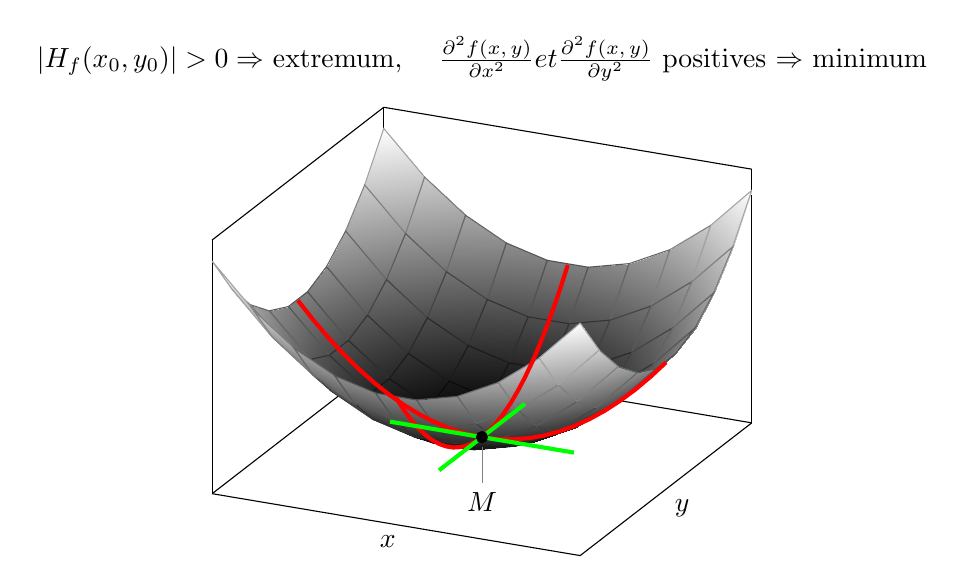
\begin{tikzpicture}
\begin{axis}[title = {$\vert \bm{H}_f(x_0,y_0)\vert > 0 \Rightarrow$ extremum, $\quad\frac{\partial^2 f(x,\,y)}{\partial x^2} \text{ et } \frac{\partial^2 f(x,\,y)}{\partial y^2}$ positives $\Rightarrow$ minimum},
    xlabel = $x$, ylabel = $y$,
    ticks=none,
	colormap/blackwhite,
	]
    \addplot3[surf,shader=faceted interp,
    domain = -1:1,
    domain y = -1:1,
    samples = 10] {x^2 + y^2};
    
    \addplot3[red,domain=-1:1,samples y=0,line width=1.5pt] (x,0,x^2);
    \addplot3[red,domain=-1:1,samples y=0,line width=1.5pt] (0,x,x^2);
    \addplot3[green,domain=-0.5:0.5,samples y=0,line width=1.5pt] (x,0,0);
    \addplot3[green,domain=-0.5:0.5,samples y=0,line width=1.5pt] (0,x,0);
    \addplot3[only marks,point meta=explicit symbolic] coordinates { (0,0,0) };
    \node[pin=-90:$M$] at (0,0,0) {};
\end{axis}
\end{tikzpicture}



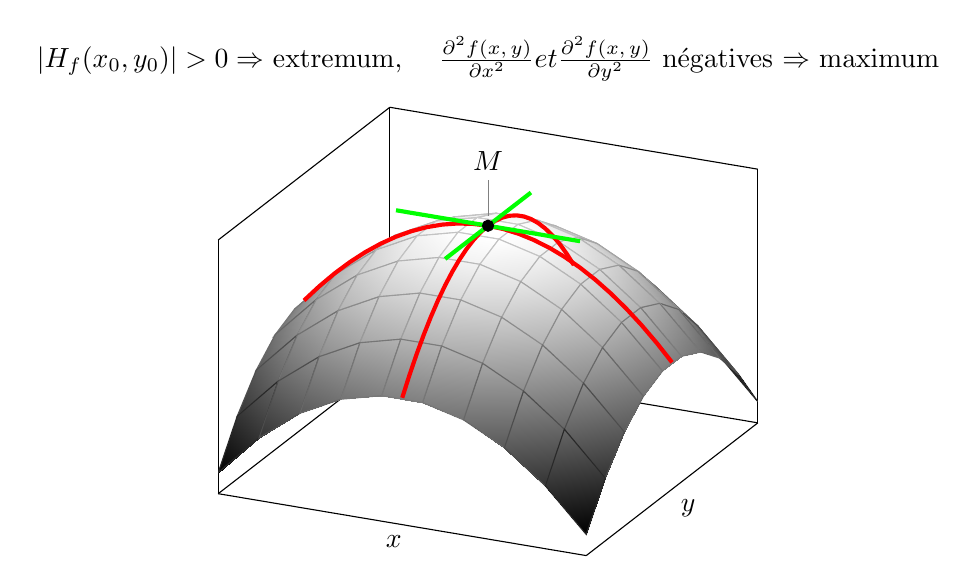
\begin{tikzpicture}
\begin{axis}[title = {$\vert \bm{H}_f(x_0,y_0)\vert > 0 \Rightarrow$ extremum, $\quad\frac{\partial^2 f(x,\,y)}{\partial x^2} \text{ et } \frac{\partial^2 f(x,\,y)}{\partial y^2}$ négatives $\Rightarrow$ maximum},
    xlabel = $x$, ylabel = $y$,
    ticks=none,
	colormap/blackwhite,
	]
    \addplot3[surf,shader=faceted interp,
    domain = -1:1,
    domain y = -1:1,
    samples = 10] {-x^2 - y^2};
    
    \addplot3[red,domain=-1:1,samples y=0,line width=1.5pt] (x,0,-x^2);
    \addplot3[red,domain=-1:1,samples y=0,line width=1.5pt] (0,x,-x^2);
    \addplot3[green,domain=-0.5:0.5,samples y=0,line width=1.5pt] (x,0,0);
    \addplot3[green,domain=-0.5:0.5,samples y=0,line width=1.5pt] (0,x,0);
    \addplot3[only marks,point meta=explicit symbolic] coordinates { (0,0,0) };
    \node[pin=90:$M$] at (0,0,0) {};
\end{axis}
\end{tikzpicture}

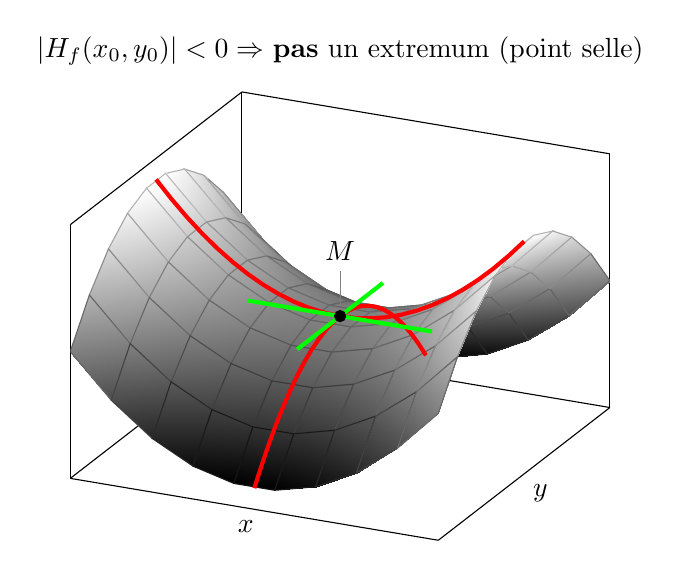
\begin{tikzpicture}
\begin{axis}[title = {$\vert \bm{H}_f(x_0,y_0)\vert < 0 \Rightarrow$ \textbf{pas} un extremum (point selle)},
    xlabel = $x$, ylabel = $y$,
    ticks=none,
	colormap/blackwhite,
	]
    \addplot3[surf,shader=faceted interp,
    domain = -1:1,
    domain y = -1:1,
    samples = 10] {x^2 - y^2};
    
    \addplot3[red,domain=-1:1,samples y=0,line width=1.5pt] (x,0,x^2);
    \addplot3[red,domain=-1:1,samples y=0,line width=1.5pt] (0,x,-x^2);
    \addplot3[green,domain=-0.5:0.5,samples y=0,line width=1.5pt] (x,0,0);
    \addplot3[green,domain=-0.5:0.5,samples y=0,line width=1.5pt] (0,x,0);
    \addplot3[only marks,point meta=explicit symbolic] coordinates { (0,0,0) };
    \node[pin=90:$M$] at (0,0,0) {};
\end{axis}
\end{tikzpicture}

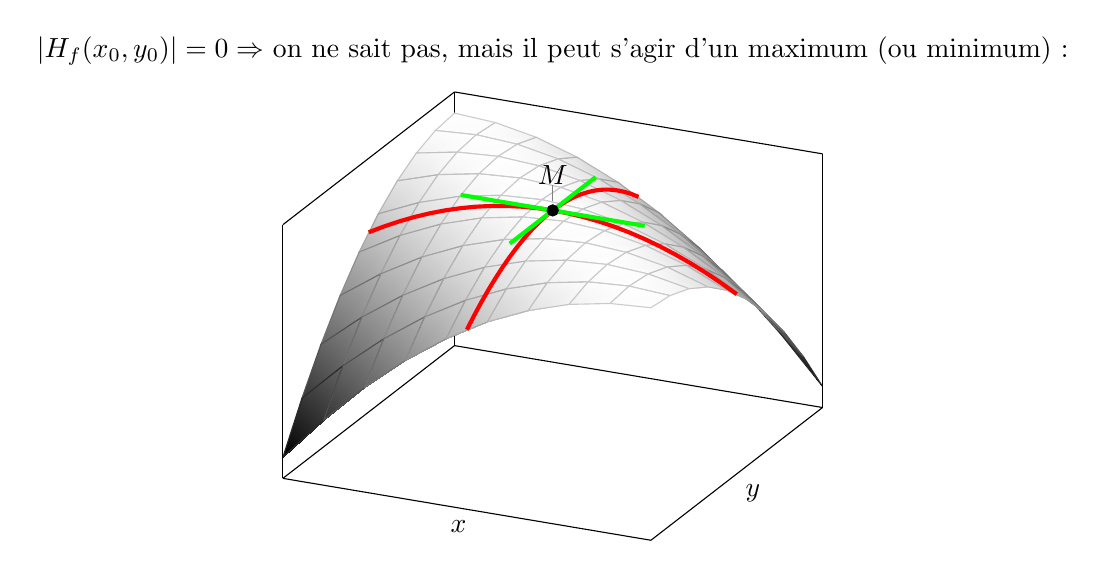
\begin{tikzpicture}
\begin{axis}[title = {$\vert \bm{H}_f(x_0,y_0)\vert = 0 \Rightarrow$ on ne sait pas, mais il peut s'agir d'un maximum (ou minimum) :},
    xlabel = $x$, ylabel = $y$,
    ticks=none,
	colormap/blackwhite,
	]
    \addplot3[surf,shader=faceted interp,
    domain = -1:1,
    domain y = -1:1,
    samples = 10] {-x^2 - y^2 -2*x*y};
    
    \addplot3[red,domain=-1:1,samples y=0,line width=1.5pt] (x,0,-x^2);
    \addplot3[red,domain=-1:1,samples y=0,line width=1.5pt] (0,x,-x^2);
    \addplot3[green,domain=-0.5:0.5,samples y=0,line width=1.5pt] (x,0,0);
    \addplot3[green,domain=-0.5:0.5,samples y=0,line width=1.5pt] (0,x,0);
    \addplot3[only marks,point meta=explicit symbolic] coordinates { (0,0,0) };
    \node[pin={[inner sep=0pt, outer sep=0pt, pin distance=0.2cm]90:$M$}] at (0,0,0) {};
\end{axis}
\end{tikzpicture}

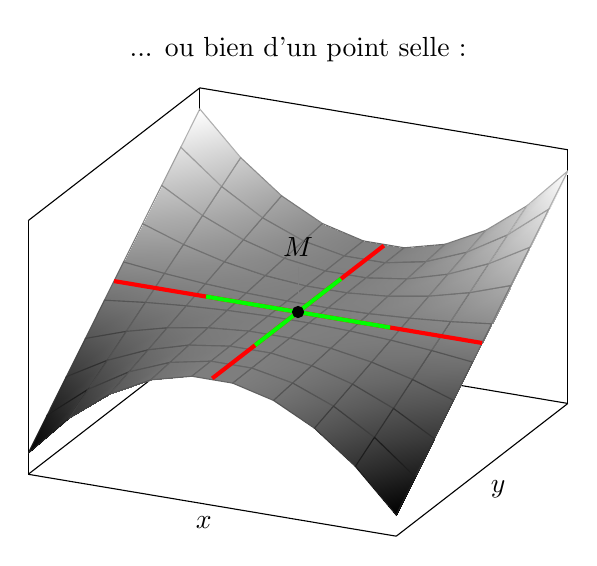
\begin{tikzpicture}
\begin{axis}[title = {... ou bien d'un point selle :},
    xlabel = $x$, ylabel = $y$,
    ticks=none,
	colormap/blackwhite,
	]
    \addplot3[surf,shader=faceted interp,
    domain = -1:1,
    domain y = -1:1,
    samples = 10] {y*x^2};
    
    \addplot3[red,domain=-1:1,samples y=0,line width=1.5pt] (x,0,0);
    \addplot3[red,domain=-1:1,samples y=0,line width=1.5pt] (0,x,0);
    \addplot3[green,domain=-0.5:0.5,samples y=0,line width=1.5pt] (x,0,0);
    \addplot3[green,domain=-0.5:0.5,samples y=0,line width=1.5pt] (0,x,0);
    \addplot3[only marks,point meta=explicit symbolic] coordinates { (0,0,0) };
    \node[pin=90:$M$] at (0,0,0) {};
\end{axis}
\end{tikzpicture}

\end{center}




\begin{exo}

\noindent Pour chacune des fonctions suivantes (toutes définies sur $\mathbb{R}^2$), calculer $\bm{\nabla} f(x,\,y)$ pour en déduire les points critiques. Pour ces points critiques, calculer le discriminant hessien pour dire si il est un extremum (si c'est le cas, préciser la valeur de $f$ et s'il s'agit d'un minimum ou d'un maximum).


\begin{tasks}(1)
\task $f(x,\,y) = x^2+y^2$
\task $f(x,\,y) = 1+x+y+x^2-xy+y^2$
\task $f(x,\,y) = x^3+y^3 + 3xy$
\end{tasks}
\end{exo}

\begin{sol}
\begin{tasks}(1)
\task $f(x,\,y) = x^2+y^2$,\\
$\bm{\nabla}f(x,\,y) = \vec{0} \Rightarrow \begin{cases} 2x &= 0 \\ 2y &= 0 \end{cases}$ donc le seul point critique est $M(0,0)$\\
$\vert \bm{H}_f (x,y)\vert =  \begin{vmatrix} r=2 & s=0 \\ s=0 & t=2\end{vmatrix} = 4 = \vert \bm{H}_f (0,0)\vert > 0$ \\
Donc $M(0,\, 0,\, 0)$ est une extremum, et comme $(r=2)>0$, il s'agit d'un minimum.\\
%
\begin{center}
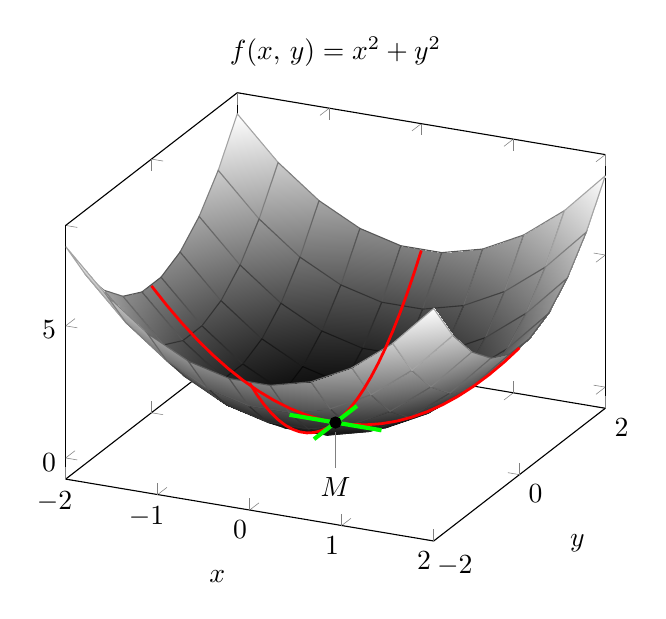
\begin{tikzpicture}
\begin{axis}[title={$f(x,\,y) = x^2+y^2$}, xlabel = $x$, ylabel = $y$,
	colormap/blackwhite,
	]
    \addplot3[surf,shader=faceted interp,
    domain = -2:2,
    domain y = -2:2,
    samples = 10] {x^2 + y^2};
    
    \addplot3[red,domain=-2:2,samples y=0,line width=1pt] (x,0,x^2);
    \addplot3[red,domain=-2:2,samples y=0,line width=1pt] (0,x,x^2);
    \addplot3[green,domain=-0.5:0.5,samples y=0,line width=1.5pt] (x,0,0);
    \addplot3[green,domain=-0.5:0.5,samples y=0,line width=1.5pt] (0,x,0);
    \node[pin=-90:$M$] at (0,0,0) {};
    
    \addplot3[only marks,point meta=explicit symbolic] coordinates { (0,0,0) };
\end{axis}
\end{tikzpicture}
\end{center}

\task $f(x,\,y) = 1+x+y+x^2-xy+y^2$,\\
$\bm{\nabla}f(x,\,y) = \vec{0} \Rightarrow \begin{cases} 1+2x-y &= 0 \\ 1 -x + 2y &= 0 \end{cases}$ donc le seul point critique est $M(-1,-1)$\\
$\vert \bm{H}_f (x,y)\vert =  \begin{vmatrix} r=2 & s=-1 \\ s=-1 & t=2\end{vmatrix} = 3 = \vert \bm{H}_f (-1,-1)\vert > 0$ \\
Donc $M(-1,-1)$ est une extremum, et comme $(r=2)>0$, il s'agit d'un minimum.\\
%
\begin{center}
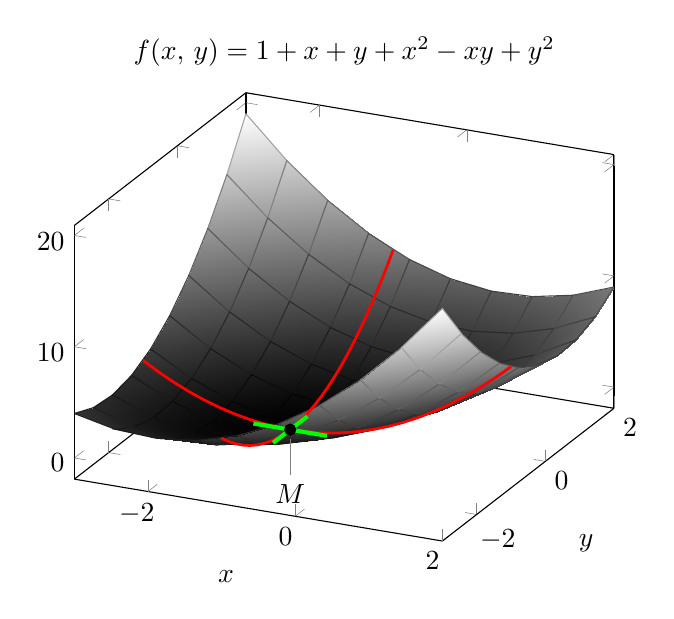
\begin{tikzpicture}
\begin{axis}[title={$f(x,\,y) = 1+x+y+x^2-xy+y^2$}, xlabel = $x$, ylabel = $y$,
	%grid,
	colormap/blackwhite,
	]
    \addplot3[surf,shader=faceted interp,
    domain = -3:2,
    domain y = -3:2,
    samples = 10] {1 + x + y + x^2 - x*y + y^2};
    
    \addplot3[red,domain=-3:2,samples y=0,line width=1pt] (x,-1,1+x-1+x^2+x+1);
    \addplot3[red,domain=-3:2,samples y=0,line width=1pt] (-1,x,x+1+x+x^2);
    \addplot3[green,domain=-1.5:-0.5,samples y=0,line width=1.5pt] (x,-1,0);
    \addplot3[green,domain=-1.5:-0.5,samples y=0,line width=1.5pt] (-1,x,0);
    \node[pin=-90:$M$] at (-1,-1,0) {};
    
    \addplot3[only marks,point meta=explicit symbolic] coordinates { (-1,-1,0) };
\end{axis}
\end{tikzpicture}
\end{center}

\task $f(x,\,y) = x^3+y^3 + 3xy$,\\
$\bm{\nabla}f(x,\,y) = \vec{0} \Rightarrow \begin{cases} 3x^2 + 3y &= 0 \\ 3y^2 + 3x  &= 0 \end{cases}$ ... $\Rightarrow x(3x^2+3) = 0 \Rightarrow x = 0 \text{ ou }-1$\\
Les valeurs de $y$ correspondantes sont respectivement 0 et -1, d'où les points critiques $A(0,0)$ et B(-1,-1).\\
$\vert \bm{H}_f (x,y)\vert =  \begin{vmatrix} r=6x & s=0 \\ s=0 & t=6y\end{vmatrix}$ \\
$\vert \bm{H}_f (0,0)\vert =  \begin{vmatrix} r=0 & s=0 \\ s=0 & t=0\end{vmatrix} = 0 \Rightarrow$ on ne sait pas.\\
$\vert \bm{H}_f (-1,-1)\vert =  \begin{vmatrix} r=-6 & s=0 \\ s=0 & t=-6\end{vmatrix} = 36 > 0 \Rightarrow B$ est un extremum.\\
Et comme $r$ et $t$ sont négatifs, $B$ est une maximum.\\
%
\begin{center}
%\begin{tikzpicture}
%\begin{axis}[title={$f(x,\,y) = x^3+y^3 + 3xy$}, xlabel = $x$, ylabel = $y$,
%	colormap/cool,
%	]
%    \addplot3[surf,shader=interp,
%    domain = -2:1,
%    domain y = -2:1,
%    samples = 30] {x^3 + y^3 + 3*x*y};
    
%    \addplot3[red,domain=-2:1,samples y=0,line width=1pt] (x,0,x^3);
%    \addplot3[red,domain=-2:1,samples y=0,line width=1pt] (0,x,x^3);
%    \addplot3[green,domain=-0.5:0.5,samples y=0,line width=1.5pt] (x,0,0);
%    \addplot3[green,domain=-0.5:0.5,samples y=0,line width=1.5pt] (0,x,0);
%    \node[pin=90:$A$] at (0,0,0) {};
    
%    \addplot3[red,domain=-2:1,samples y=0,line width=1pt] (x,-1,x^3-1-3*x);
%    \addplot3[red,domain=-2:1,samples y=0,line width=1pt] (-1,x,-1+x^3-3*x);
%    \addplot3[green,domain=-1.5:-0.5,samples y=0,line width=1.5pt] (x,-1,1);
%    \addplot3[green,domain=-1.5:-0.5,samples y=0,line width=1.5pt] (-1,x,1);
%    \node[pin=90:$B$] at (-1,-1,1) {};
    
%    \addplot3[only marks,point meta=explicit symbolic] coordinates { (0,0,0) (-1,-1,1) };
%\end{axis}
%\end{tikzpicture}


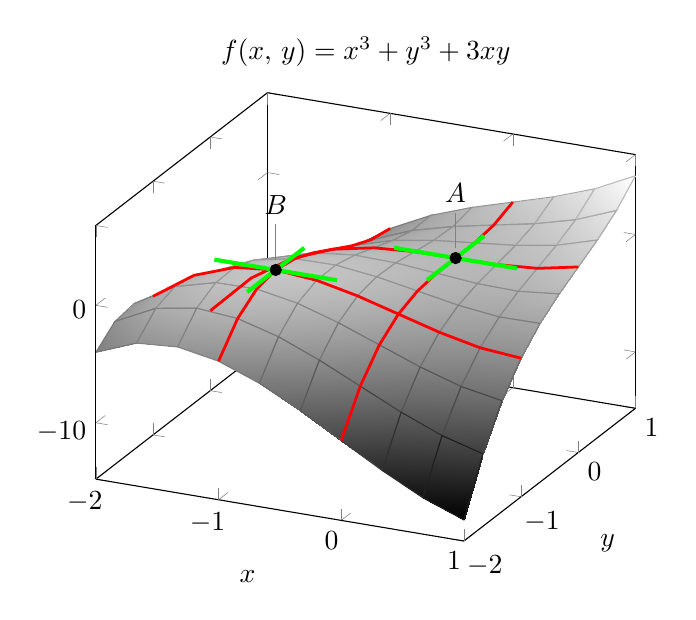
\begin{tikzpicture}
\begin{axis}[
    title={$f(x,\,y) = x^3+y^3 + 3xy$},
    xlabel=$x$,
    ylabel=$y$,
    colormap/blackwhite,
    samples=10, % Réduction du nombre d'échantillons
    shader=faceted interp, % Utilisation de faceted interp pour un rendu plus rapide
    %grid=none, % Désactive la grille
    %axis lines=center, % Affiche uniquement les axes
    %ticks=none, % Masque les graduations (optionnel)
]
    \addplot3[surf,
    domain=-2:1,
    domain y=-2:1,
    ] {x^3 + y^3 + 3*x*y};

    \addplot3[red,domain=-2:1,samples y=0,line width=1pt] (x,0,x^3);
    \addplot3[red,domain=-2:1,samples y=0,line width=1pt] (0,x,x^3);
    \addplot3[green,domain=-0.5:0.5,samples y=0,line width=1.5pt] (x,0,0);
    \addplot3[green,domain=-0.5:0.5,samples y=0,line width=1.5pt] (0,x,0);
    \node[pin=90:$A$] at (0,0,0) {};

    \addplot3[red,domain=-2:1,samples y=0,line width=1pt] (x,-1,x^3-1-3*x);
    \addplot3[red,domain=-2:1,samples y=0,line width=1pt] (-1,x,-1+x^3-3*x);
    \addplot3[green,domain=-1.5:-0.5,samples y=0,line width=1.5pt] (x,-1,1);
    \addplot3[green,domain=-1.5:-0.5,samples y=0,line width=1.5pt] (-1,x,1);
    \node[pin=90:$B$] at (-1,-1,1) {};

    \addplot3[only marks,samples=9] coordinates { (0,0,0) (-1,-1,1) };
\end{axis}
\end{tikzpicture}


\end{center}

\end{tasks}
\end{sol}


\begin{exo}

\noindent \ding{45} Même exercice pour les fonctions suivantes qui ont un domaine de définition plus compliqué.


\begin{tasks}(1)
\task $f(x,\,y) = \displaystyle \frac{1}{1-x} + \frac{1}{1-y} + \frac{1}{x+y}$, pour les points critiques $A(-1,\ -1)$; $B(-1,\ 3)$, $C(3,\ -1)$ et $D(1/3,\ 1/3)$
\task $f(x,\,y) = x(\ln^2 x + y^2)$
\task $f(x,\,y) = \displaystyle \frac{2(x+y) + 1}{xy}$
\end{tasks}
\end{exo}

\begin{sol}
\begin{tasks}(1)
\task $f(x,\,y) = \displaystyle \frac{1}{1-x} + \frac{1}{1-y} + \frac{1}{x+y}$, pour les points critiques $A(-1,\,-1)$; $B(-1,\,3)$, $C(3,\,-1)$ et $D(1/3,\,1/3)$\\
Notons que ces droites dans le plan $Oxy$ sont exclues de l'ensemble de définition : $x=1$, $y=1$ et $y=-x$.\\
On pourra vérifier, pour les points $A$ à $D$ que $\bm{\nabla} f(x,\,y) = \vec{0}$ avec :
$$\frac{\partial}{\partial x} f(x,\,y) = \frac{1}{(1-x)^2}  - \frac{1}{(x+y)^2}$$
$$\frac{\partial}{\partial y} f(x,\,y) = \frac{1}{(1-y)^2}  - \frac{1}{(x+y)^2}$$
La matrice hessienne est calculée à partir des relations suivantes :
$$r(x,y)=\frac{\partial^2}{\partial x^2} f(x,\,y) = \frac{2}{(1-x)^3}  + \frac{2}{(x+y)^3}$$
$$t(x,y)=\frac{\partial^2}{\partial y^2} f(x,\,y) = \frac{2}{(1-y)^3}  + \frac{2}{(x+y)^3}$$
$$s(x,y)=\frac{\partial^2}{\partial x \partial y} f(x,\,y) = \frac{2}{(x+y)^3}$$
Donc\\
$\vert \bm{H}_f (-1,-1)\vert =  \begin{vmatrix} r=0 & s=-2/8 \\ s=-2/8 & t=0\end{vmatrix} = -1/16 < 0 \Rightarrow A$ n'est pas un extremum.\\
$\vert \bm{H}_f (-1,3)\vert =  \begin{vmatrix} r=4/8 & s=2/8 \\ s=2/8 & t=0\end{vmatrix} = -1/16 < 0 \Rightarrow B$ n'est pas un extremum.\\
$\vert \bm{H}_f (3,-1)\vert =  \begin{vmatrix} r=0 & s=2/8 \\ s=2/8 & t=4/8\end{vmatrix} = -1/16 < 0 \Rightarrow C$ n'est pas un extremum.\\
$\vert \bm{H}_f (\frac{1}{3},\frac{1}{3})\vert =  \begin{vmatrix} r=27/2 & s=27/4 \\ s=27/4 & t=27/2\end{vmatrix} = \frac{2187}{16} > 0 \Rightarrow D$ est un minimum local à $f(1/3,1/3)=9/2$.\\
%
\begin{center}
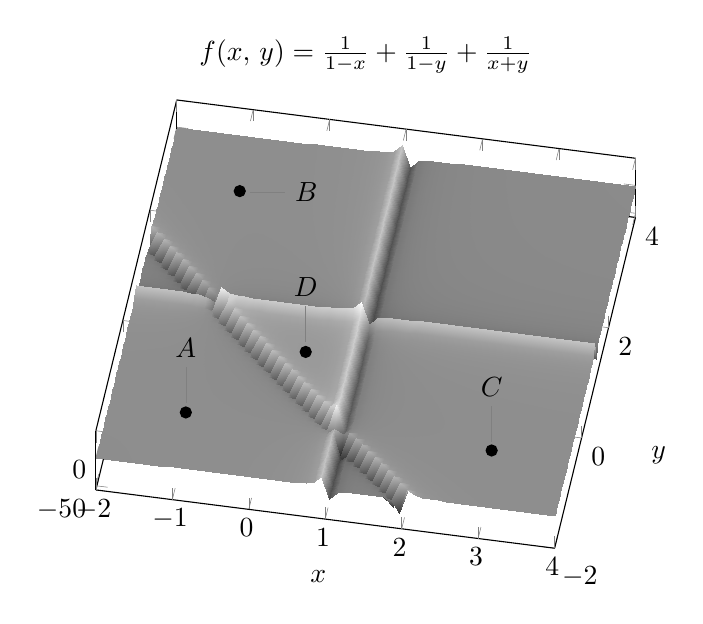
\begin{tikzpicture}
\begin{axis}[title={$f(x,\,y) = \frac{1}{1-x} + \frac{1}{1-y} + \frac{1}{x+y}$}, xlabel = $x$, ylabel = $y$,
	%grid,
	colormap/blackwhite,
    view={10}{80},
	]
    \addplot3[surf,shader=interp,samples=60,
    domain = -2:4,
    domain y = -2:4] {1/(1-x) + 1/(1-y) + 1/(x+y)};
    
    \node[pin=90:$A$] at (-1,-1,0) {};
    \node[pin=0:$B$] at (-1,3,0) {};
    \node[pin=90:$C$] at (3,-1,0) {};
    \node[pin=90:$D$] at (0.333,0.333,0) {};
    
    \addplot3[only marks,point meta=explicit symbolic] coordinates { (-1,-1,0) (-1,3,1.5) (3,-1,1.5) (0.333,0.333,0) };
\end{axis}
\end{tikzpicture}
\end{center}


\task $f(x,\,y) = x(\ln^2 x + y^2)$, domaine de définition = $x>0$ et $y \in \mathbb{R}$
$$\frac{\partial}{\partial x} f(x,\,y) = \left( \ln^2 x  + y^2\right)  + \left( x \times 2\ln x \frac{1}{x}\right)= \ln^2 x + 2\ln x + y^2$$
$$\frac{\partial}{\partial y} f(x,\,y) = 2xy$$
Si $2xy = 0$ alors soit $x=0$, soit $y=0$, mais puisque $x>0$, la seule solution est $\boxed{y=0}$.\\
Dans la première équation, en prenant $y=0$, on obtient $\ln^2 x + 2\ln x = 0$.\\
Changement de variable $X=\ln x$ donne $X^2+2X = 0$ qui a pour solution $0$ ou $-2$.\\
$$X = 0 \Rightarrow \ln x = 0 \Rightarrow \boxed{x = 1}$$ 
$$X = -2 \Rightarrow \ln x = -2 \Rightarrow \boxed{x = e^{-2}}$$
Les points critiques sont donc $A(1,0)$ et $B(e^{-2},0)$.\\
La matrice hessienne est calculée à partir des relations suivantes :
$$r(x,y)=\frac{\partial^2}{\partial x^2} f(x,\,y) = \frac{2(\ln x +1)}{x}$$
$$t(x,y)=\frac{\partial^2}{\partial y^2} f(x,\,y) = 2x$$
$$s(x,y)=\frac{\partial^2}{\partial x \partial y} f(x,\,y) = 2y$$
Donc\\
$\vert \bm{H}_f (1,0)\vert =  \begin{vmatrix} r=2 & s=0 \\ s=0 & t=2\end{vmatrix} = 4 > 0 \Rightarrow A$ est un minimum.\\
$\vert \bm{H}_f (e^{-2},0)\vert =  \begin{vmatrix} r=-2e^{2} & s=0 \\ s=0 & t=2e^{-2}\end{vmatrix} = -4 < 0 \Rightarrow B$ pas un extremum.\\
%
\begin{center}
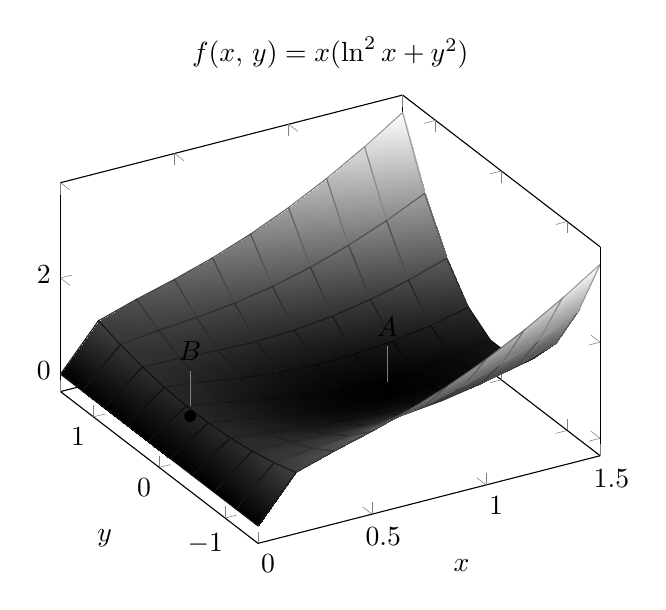
\begin{tikzpicture}
\begin{axis}[title={$f(x,\,y) = x(\ln^2 x + y^2)$}, xlabel = $x$, ylabel = $y$,
	%grid,
	colormap/blackwhite,
    view={-30}{40},
	]
    \addplot3[surf,shader=faceted interp,samples=10,
    domain = 0:1.5,
    domain y = -1.5:1.5] {x*(ln(x)*ln(x) + y^2) };
    
    \node[pin=90:$A$] at (1,0,0) {};
    \node[pin=90:$B$] at (0.13533,0,0.54132) {};
    
    \addplot3[only marks,point meta=explicit symbolic] coordinates { (1,0,0) (0.13533,0,0.54132) };
\end{axis}
\end{tikzpicture}
\end{center}

\task $f(x,\,y) = \displaystyle \frac{2(x+y) + 1}{xy}$, $x\ne0$ et $y\ne0$
$$\frac{\partial}{\partial x} f(x,\,y) = -\frac{2y+1}{x^2y}$$
$$\frac{\partial}{\partial y} f(x,\,y) = -\frac{2x+1}{xy^2}$$
Le seul point critique est $A(-\frac{1}{2},-\frac{1}{2})$ 
$$r(x,y)=\frac{\partial^2}{\partial x^2} f(x,\,y) = \frac{4y+2}{x^3y}$$
$$t(x,y)=\frac{\partial^2}{\partial y^2} f(x,\,y) =  \frac{4x+2}{xy^3}$$
$$s(x,y)=\frac{\partial^2}{\partial x \partial y} f(x,\,y) = \frac{1}{(xy)^2}$$
Donc\\
$\vert \bm{H}_f (-1/2,-1/2)\vert =  \begin{vmatrix} r=0 & s=16 \\ s=16 & t=0\end{vmatrix} = 16^2 < 0 \Rightarrow A$ pas extremum.\\
%
\begin{center}
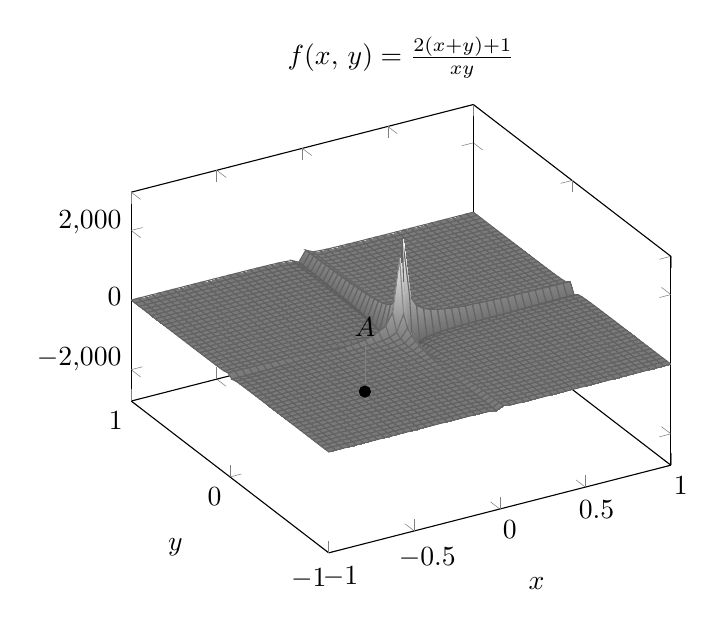
\begin{tikzpicture}
\begin{axis}[
    title={$f(x,\,y) = \frac{2(x+y) + 1}{xy}$}, 
    xlabel = $x$, ylabel = $y$,	
    view={-30}{40},
    colormap/blackwhite
    ]
    \addplot3[surf,shader=faceted interp,samples=50,
    domain = -1.:1.,
    domain y = -1.:1.] {(2*(x+y) + 1)/(x*y)};
    
    \node[pin=90:$A$] at (-0.5,-0.5,12) {};
    
    \addplot3[only marks,point meta=explicit symbolic] coordinates { (-0.5,-0.5,12) };
\end{axis}
\end{tikzpicture}
\end{center}


\end{tasks}
\end{sol}

